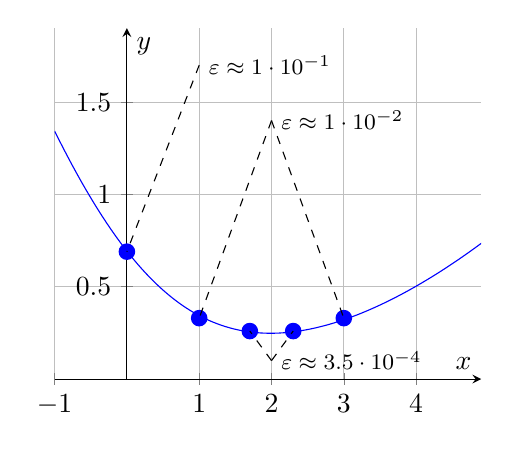
\begin{tikzpicture}
\begin{axis}[
    width=7cm,
    xlabel={$x$},
    ylabel={$y$},
    xmin=-1, xmax=4.9,
    ymin=-0, ymax=1.9,
    axis lines=center,
    grid=both,
    samples=100,
]
\addplot[blue, domain=-1:5] {-ln(1/(1 + exp(-x))) + x^2/33};

\coordinate (A1) at (axis cs:1, 0.33);
\coordinate (B1) at (axis cs:2, 1.4);
\coordinate (C1) at (axis cs:3,0.33);

\fill[blue, thick] (A1) circle (3pt);
\fill[blue, thick] (C1) circle (3pt);
\node[right] at (B1) {\footnotesize $\bm{\varepsilon \approx 1 \cdot 10^{-2}}$};

\draw[dashed] (B1) -- (A1);
\draw[dashed] (B1) -- (C1);
 %----------------------------------------%
\coordinate (A2) at (axis cs:1.7, 0.26);
\coordinate (B2) at (axis cs:2, 0.1);
\coordinate (C2) at (axis cs:2.3,  0.26);

\fill[blue, thick] (A2) circle (3pt);
\fill[blue, thick] (C2) circle (3pt);
\node[right] at (B2) {\footnotesize $ \bm{\varepsilon \approx 3.5 \cdot 10^{-4}}$};

\draw[dashed] (B2) -- (A2);
\draw[dashed] (B2) -- (C2);
 %----------------------------------------%
 \coordinate (A2) at (axis cs:0, 0.69);
\coordinate (B2) at (axis cs:1, 1.7);

\fill[blue, thick] (A2) circle (3pt);
\node[right] at (B2) {\footnotesize $\bm{\varepsilon \approx 1 \cdot 10^{-1}}$};

\draw[dashed] (B2) -- (A2);
 %----------------------------------------%
\end{axis}
\end{tikzpicture}